\begin{figure}[h]
\begin{minipage}{0.49\textwidth}
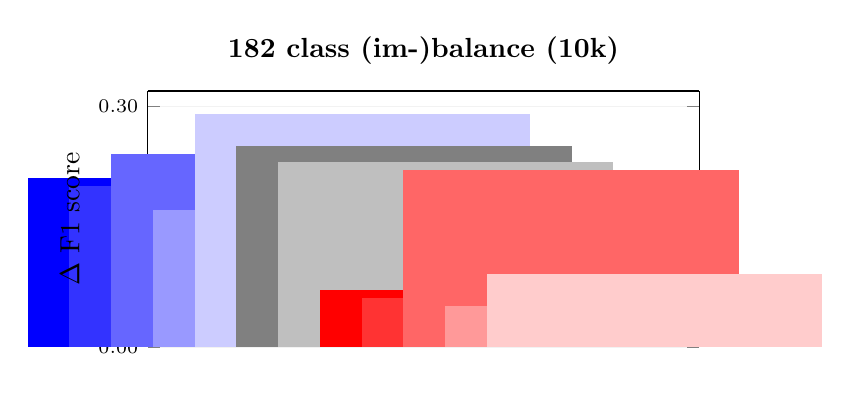
\begin{tikzpicture}
	\begin{axis}[
    		title=\textbf{\ding{182} class (im-)balance (10k)},
		ylabel=$\Delta$ F1 score,
		scale only axis,
		clip=false,
		separate axis lines,
		xtick={1,2,3,4,5,6,7,8,9,10,11,12},
        	x tick style={draw=none},
        	xticklabels={Average,p-Means,SIF,GEM,Hier. pooling,BOREP,rand. BiLSTM,InferSent,Quick-Th.,sent2vec,BERT,LASER},
		xticklabels={,,},
		width=7cm,height=3.25cm,
		tick label style={font=\scriptsize},
		xticklabel style={rotate=90},
		ymajorgrids,
    		grid style={line width=.1pt, draw=gray!10},
		ymin=0,
		every axis plot/.append style={
          		ybar,
          		bar width=8.0,
          		bar shift=0.5pt,
			fill
		},
		scaled y ticks=false,
		y tick label style={
        		/pgf/number format/.cd,
            		fixed,
            		fixed zerofill,
            		precision=2,
        		/tikz/.cd
    		}
	]

		\addplot[blue] coordinates {(1,0.21)};
     	 	\addplot[blue!80] coordinates {(2,0.20)};
      		\addplot[blue!60] coordinates {(3,0.24)};
      		\addplot[blue!40] coordinates {(4,0.17)};
		\addplot[blue!20] coordinates {(5,0.29)};
     	 	\addplot[gray] coordinates {(6,0.25)};
      		\addplot[lightgray] coordinates {(7,0.23)};
      		\addplot[red] coordinates {(8,0.07)};
     	 	\addplot[red!80] coordinates {(9,0.06)};
      		\addplot[red!60] coordinates {(10,0.22)};
      		\addplot[red!40] coordinates {(11,0.05)};
		\addplot[red!20] coordinates {(12,0.09)};
	\end{axis}
\end{tikzpicture}
\end{minipage}
\hfill
\begin{minipage}{0.49\textwidth}
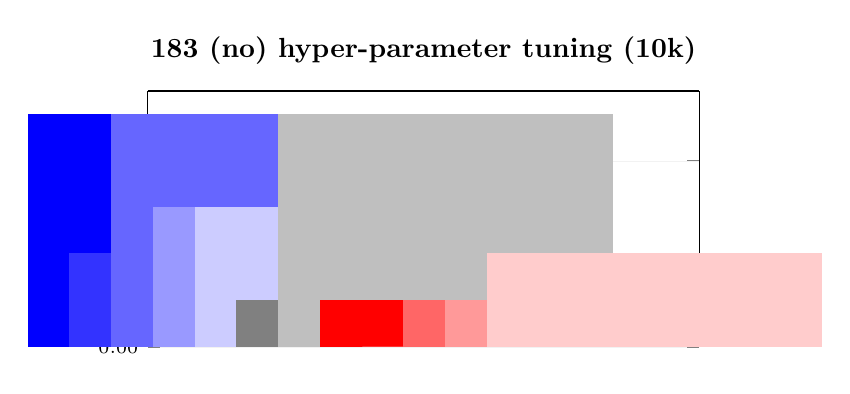
\begin{tikzpicture}
	\begin{axis}[
    		title=\textbf{\ding{183} (no) hyper-parameter tuning (10k)},
		scale only axis,
		clip=false,
		separate axis lines,
		xtick={1,2,3,4,5,6,7,8,9,10,11,12},
        	x tick style={draw=none},
        	xticklabels={Average,p-Means,SIF,GEM,Hier. pooling,BOREP,rand. BiLSTM,InferSent,Quick-Th.,sent2vec,BERT,LASER},
		xticklabels={,,},
		width=7cm,height=3.25cm,
		tick label style={font=\scriptsize},
		xticklabel style={rotate=90},
		ymajorgrids,
    		grid style={line width=.1pt, draw=gray!10},
		ymin=0,
		every axis plot/.append style={
          		ybar,
          		bar width=8.0,
          		bar shift=0.5pt,
			fill
		},
		scaled y ticks=false,
		y tick label style={
        		/pgf/number format/.cd,
            		fixed,
            		fixed zerofill,
            		precision=2,
        		/tikz/.cd
    		}
	]

		\addplot[blue] coordinates {(1,0.05)};
     	 	\addplot[blue!80] coordinates {(2,0.02)};
      		\addplot[blue!60] coordinates {(3,0.05)};
      		\addplot[blue!40] coordinates {(4,0.03)};
		\addplot[blue!20] coordinates {(5,0.03)};
     	 	\addplot[gray] coordinates {(6,0.01)};
      		\addplot[lightgray] coordinates {(7,0.05)};
      		\addplot[red] coordinates {(8,0.01)};
     	 	\addplot[red!80] coordinates {(9,0.00)};
      		\addplot[red!60] coordinates {(10,0.01)};
      		\addplot[red!40] coordinates {(11,0.01)};
		\addplot[red!20] coordinates {(12,0.02)};
	\end{axis}
\end{tikzpicture}
\end{minipage}

\begin{minipage}{0.49\textwidth}
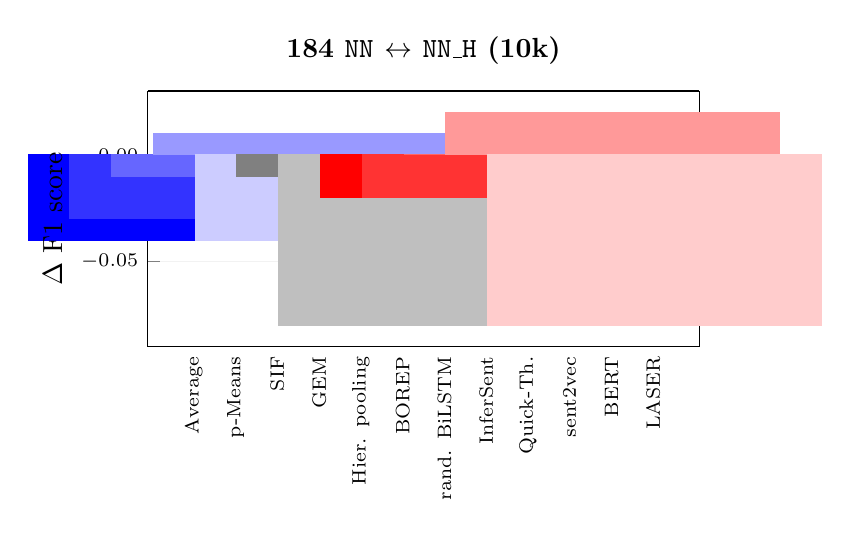
\begin{tikzpicture}
	\begin{axis}[
    		title=\textbf{\ding{184} \texttt{NN} $\leftrightarrow$ \texttt{NN\_H} (10k)},
		ylabel=$\Delta$ F1 score,
		scale only axis,
		clip=false,
		separate axis lines,
		xtick={1,2,3,4,5,6,7,8,9,10,11,12},
        	x tick style={draw=none},
        	xticklabels={Average,p-Means,SIF,GEM,Hier. pooling,BOREP,rand. BiLSTM,InferSent,Quick-Th.,sent2vec,BERT,LASER},
		width=7cm,height=3.25cm,
		tick label style={font=\scriptsize},
		xticklabel style={rotate=90},
		ymajorgrids,
    		grid style={line width=.1pt, draw=gray!10},
		every axis plot/.append style={
          		ybar,
          		bar width=8.0,
          		bar shift=0.5pt,
			fill
		},
		scaled y ticks=false,
		y tick label style={
        		/pgf/number format/.cd,
            		fixed,
            		fixed zerofill,
            		precision=2,
        		/tikz/.cd
    		}
	]

		\addplot[blue] coordinates {(1,-0.04)};
     	 	\addplot[blue!80] coordinates {(2,-0.03)};
      		\addplot[blue!60] coordinates {(3,-0.01)};
      		\addplot[blue!40] coordinates {(4,0.01)};
		\addplot[blue!20] coordinates {(5,-0.04)};
     	 	\addplot[gray] coordinates {(6,-0.01)};
      		\addplot[lightgray] coordinates {(7,-0.08)};
      		\addplot[red] coordinates {(8,-0.02)};
     	 	\addplot[red!80] coordinates {(9,-0.02)};
      		\addplot[red!60] coordinates {(10,0.00)};
      		\addplot[red!40] coordinates {(11,0.02)};
		\addplot[red!20] coordinates {(12,-0.08)};
	\end{axis}
\end{tikzpicture}
\end{minipage}
\hfill
\begin{minipage}{0.49\textwidth}
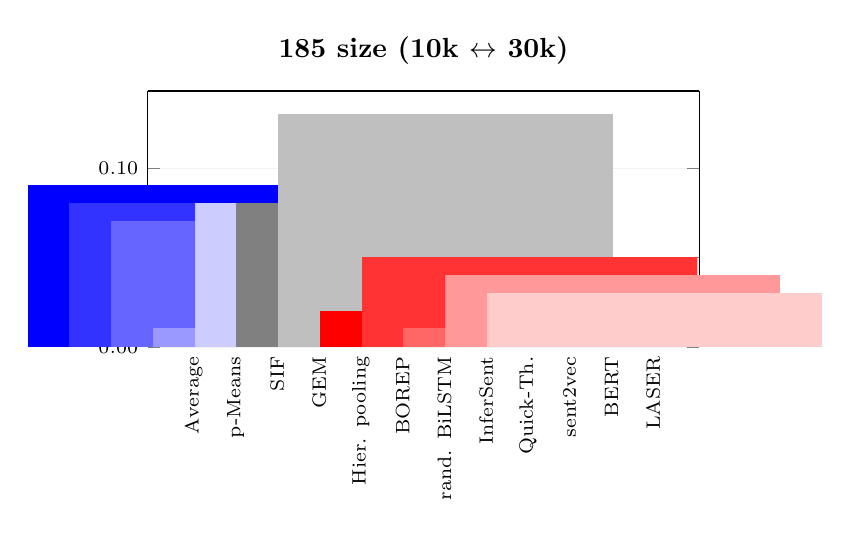
\begin{tikzpicture}
	\begin{axis}[
    		title=\textbf{\ding{185} size (10k $\leftrightarrow$ 30k)},
		scale only axis,
		clip=false,
		separate axis lines,
		xtick={1,2,3,4,5,6,7,8,9,10,11,12},
        	x tick style={draw=none},
        	xticklabels={Average,p-Means,SIF,GEM,Hier. pooling,BOREP,rand. BiLSTM,InferSent,Quick-Th.,sent2vec,BERT,LASER},
		width=7cm,height=3.25cm,
		tick label style={font=\scriptsize},
		xticklabel style={rotate=90},
		ymajorgrids,
    		grid style={line width=.1pt, draw=gray!10},
		ymin=0,
		every axis plot/.append style={
          		ybar,
          		bar width=8.0,
          		bar shift=0.5pt,
			fill
		},
		scaled y ticks=false,
		y tick label style={
        		/pgf/number format/.cd,
            		fixed,
            		fixed zerofill,
            		precision=2,
        		/tikz/.cd
    		}
	]

		\addplot[blue] coordinates {(1,0.09)};
     	 	\addplot[blue!80] coordinates {(2,0.08)};
      		\addplot[blue!60] coordinates {(3,0.07)};
      		\addplot[blue!40] coordinates {(4,0.01)};
		\addplot[blue!20] coordinates {(5,0.08)};
     	 	\addplot[gray] coordinates {(6,0.08)};
      		\addplot[lightgray] coordinates {(7,0.13)};
      		\addplot[red] coordinates {(8,0.02)};
     	 	\addplot[red!80] coordinates {(9,0.05)};
      		\addplot[red!60] coordinates {(10,0.01)};
      		\addplot[red!40] coordinates {(11,0.04)};
		\addplot[red!20] coordinates {(12,0.03)};
	\end{axis}
\end{tikzpicture}
\end{minipage}
\caption[Absolute F1 performance deltas in the \caps{WC} task (\texttt{NN\_H})]
	{Absolute F1 performance deltas in the \caps{WC} task (\texttt{NN\_H}):
	\ding{182} Effect of \texttt{class balance} (positive number indicates positive effect of balanced data),
	\ding{183} Effect of \texttt{hyper-parameter tuning} (on balanced data),
	\ding{184} Effect of \texttt{classifier} (on balanced data; negative values indicate worse performance of \texttt{NN}) and
	\ding{185} effect of \texttt{size} (on balanced data sets).}
\label{fig:wc_detail_deltas}
\end{figure}